\documentclass[tikz,border=8pt]{standalone}
\usepackage{amsmath,amssymb}
\usetikzlibrary{arrows.meta,calc,decorations.markings,decorations.pathmorphing,patterns,shapes.geometric,positioning}
\begin{document}
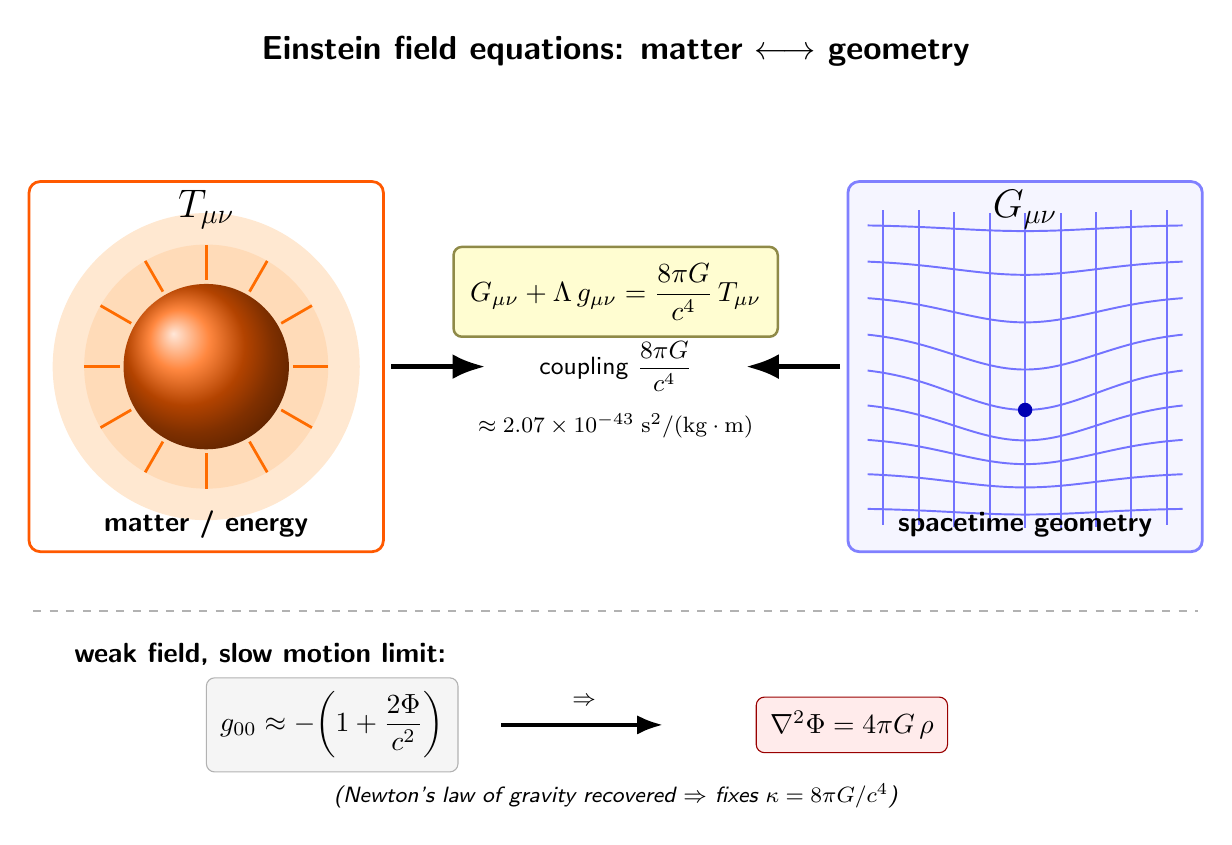
\begin{tikzpicture}[>=Latex, font=\sffamily]

% --- title ---
\node[font=\sffamily\bfseries\large] at (0,5.6)
  {Einstein field equations: matter $\longleftrightarrow$ geometry};

% =========================================================
% LEFT BLOCK: matter T_{mu nu} (orange/red sun)
% =========================================================
\begin{scope}[shift={(-5.2,1.6)}]

  % glow halo
  \fill[orange!18] (0,0) circle (1.95);
  \fill[orange!28] (0,0) circle (1.55);

  % sun core
  \shade[ball color=orange!75!red] (0,0) circle (1.05);

  % rays
  \foreach \a in {0,30,60,...,330}{
    \draw[orange!85!red,line width=1pt]
      (\a:1.1) -- (\a:1.55);
  }

  % box
  \draw[orange!70!red,line width=1pt,rounded corners=4pt]
    (-2.25,-2.35) rectangle (2.25,2.35);

  % labels
  \node[font=\sffamily\bfseries] at (0,-2.0)
    {matter / energy};
  \node[font=\Large] at (0,2.0) {$T_{\mu\nu}$};

\end{scope}

% =========================================================
% RIGHT BLOCK: spacetime curvature G_{mu nu} (light blue grid)
% =========================================================
\begin{scope}[shift={(5.2,1.6)}]

  % box bg
  \fill[blue!4,rounded corners=4pt]
    (-2.25,-2.35) rectangle (2.25,2.35);
  \draw[blue!50,line width=1pt,rounded corners=4pt]
    (-2.25,-2.35) rectangle (2.25,2.35);

  % curved grid (warped by mass at center)
  \foreach \i in {-4,-3,-2,-1,0,1,2,3,4}{
    \draw[blue!55,line width=0.7pt]
      plot[domain=-2:2,samples=60]
        (\x, {0.45*\i - 0.55*exp(-0.6*((\x)^2 + (0.45*\i)^2))});
  }
  \foreach \i in {-4,-3,-2,-1,0,1,2,3,4}{
    \draw[blue!55,line width=0.7pt]
      plot[domain=-2:2,samples=60]
        (0.45*\i, {\x - 0.55*exp(-0.6*((0.45*\i)^2 + (\x)^2))});
  }

  % central dimple dot
  \fill[blue!70!black] (0,-0.55) circle (2.6pt);

  % labels
  \node[font=\sffamily\bfseries] at (0,-2.0)
    {spacetime geometry};
  \node[font=\Large] at (0,2.0) {$G_{\mu\nu}$};

\end{scope}

% =========================================================
% MIDDLE: bidirectional arrow + coupling
% =========================================================
\draw[line width=2.0pt,->,>=Latex,black]
  (-2.85,1.6) -- (-1.65,1.6);
\draw[line width=2.0pt,->,>=Latex,black]
  (2.85,1.6) -- (1.65,1.6);

% formula box (yellow)
\node[draw=yellow!50!black,fill=yellow!18,line width=0.9pt,
      rounded corners=3pt,inner sep=6pt,
      font=\sffamily] at (0,2.55)
  {$\displaystyle G_{\mu\nu}+\Lambda\, g_{\mu\nu}=\frac{8\pi G}{c^{4}}\,T_{\mu\nu}$};

\node[font=\sffamily\small] at (0,1.6)
  {coupling $\dfrac{8\pi G}{c^{4}}$};

\node[font=\sffamily\footnotesize\itshape] at (0,0.85)
  {$\approx 2.07\times 10^{-43}\;\mathrm{s^{2}/(kg\cdot m)}$};

% =========================================================
% BOTTOM: weak field limit -> Poisson
% =========================================================

% horizontal divider
\draw[gray!60,dashed,line width=0.7pt]
  (-7.4,-1.5) -- (7.4,-1.5);

% weak field tag
\node[font=\sffamily\bfseries,anchor=west] at (-7.0,-2.05)
  {weak field, slow motion limit:};

% g_00 expression
\node[draw=gray!60,fill=gray!8,rounded corners=3pt,inner sep=5pt,
      font=\sffamily] at (-3.6,-2.95)
  {$g_{00}\approx -\!\left(1+\dfrac{2\Phi}{c^{2}}\right)$};

% arrow
\draw[line width=1.4pt,->,>=Latex] (-1.45,-2.95) -- (0.6,-2.95);
\node[font=\sffamily\footnotesize] at (-0.4,-2.65) {$\Rightarrow$};

% Poisson
\node[draw=red!60!black,fill=red!8,rounded corners=3pt,inner sep=5pt,
      font=\sffamily] at (3.0,-2.95)
  {$\nabla^{2}\Phi = 4\pi G\,\rho$};

\node[font=\sffamily\footnotesize\itshape] at (0,-3.85)
  {(Newton's law of gravity recovered $\Rightarrow$ fixes $\kappa = 8\pi G/c^{4}$)};

\end{tikzpicture}
\end{document}
